% Usage: knitr slide


\chapter{Multiple Groups}
\section{Examples}

\bi
  \item Compare baseline characteristics (e.g. age, height, BMI) or
    study response variable among subjects enrolled in one of three
    (or more) nonrandomized clinical trial arms
  \item Determine if pulmonary function, as measured by the forced
    expiratory volume in one second, differs in non-smokers, passive
    smokers, light smokers, and heavy smokers 
  \item Evaluate differences in artery dilation among wild type,
    knockout, and knockout+treated mice 
  \bi
    \item Could add second factor: Normoxic (normal oxygen) or hypoxic
      (insufficient oxygen) environmental conditions (a
      \textit{two-way} ANOVA) 
  \ei
  \item In general, studies with a continuous outcome and categorical
    predictors 
\ei


\section{The $k$-Sample Problem} \ems{9}\ros{12}
\bi
\item When $k=2$ we compare two means or medians, etc.
\item When $k>2$ we could do all possible pairwise 2-sample tests but
  this can be misleading and may $\uparrow$ type I error
\item Advantageous to get a single statistic testing $H_{0}$: all
  groups have the same distribution (or at least the same central
  tendency)
\ei

\section{Parametric ANOVA}
\subsection{Model}
\bi
\item Notation
  \bi 
   \item $k$ groups (samples) each from a normal distribution
   \item Population means $\mu_{1}, \mu_{2}, \ldots, \mu_{k}$
   \item $n_i$ observations from the $i$th group
   \item $y_{ij}$ is the $j$th observation from $i$th group
  \ei
\item Model specification
  \bi
    \item $y_{ij} = \mu + \alpha_i + e_{ij}$
    \item $\mu$ is a constant
    \item $\alpha_i$ is a constant specific to group $i$
    \item $e_{ij}$ is the error term, which is assumed to follow a Normal distribution with mean 0 and variance $\sigma^2$
    \item This model is overparameterized; that is, it is not possible to estimate $\mu$ and each $\alpha_i$ (a total of $k + 1$) terms using only $k$ means
  \ei
\item Restriction 1: $\Sigma \alpha_i = 0$
  \bi
    \item $\mu$ is the mean of all groups taken together, the grand or overall mean
    \item each $\alpha_i$ represents the deviation of the mean of the $i$th group from the overall mean
    \item $\epsilon_{ij}$ is the deviation of individual data points from $\mu + \alpha_i$ 
  \ei
\item Restriction 2: $\alpha_1 = 0$
  \bi
    \item $\mu$ is the mean of group 1
    \item each $\alpha_i$ represents the deviation of the mean of the $i$th group from the group 1 mean
    \item $\epsilon_{ij}$ is the deviation of individual data points from $\mu + \alpha_i$
  \ei
\item Other restrictions possible, and will vary by software package
\ei

\subsection{Hypothesis test}

\bi 
\item Hypothesis test
  \bi
    \item $H_{0}: \mu_{1}=\mu_{2}=\ldots=\mu_{k}$
    \item $H_{1}:$ at least two of the population means differ
  \ei
\item Not placing more importance on any particular pair or
  combination although large samples get more weight in the analysis
\item Assume that each of the $k$ populations has the same $\sigma$
\item If $k=2$ ANOVA yields identical $P$-value as 2-tailed 2-sample
  $t$-test
\item ANOVA uses an $F$ statistic and is always 2-tailed
\item $F$ ratio is proportional to the sum of squared differences
  between each sample mean and the grand mean over samples, divided by
  the sum of squared differences between all raw values and the mean
  of the sample from which the raw value came
\item This is the SSB/SSW (sum of squares between / sum of squares
  within)
\item SSB is identical to regression sum of squares \\
 SSW is identical to sum of squared errors in regression
\item $F=MSB/MSW$ where
 \bi
 \item MSB = mean square between = SSB/$(k-1), k-1=$ ``between group
   d.f.''
 \item MSW = mean square within = SSW/$(n-k), n-k=$ ``within group
   d.f.''
 \item Evidence for different $\mu$s $\uparrow$ when differences in
   sample means (ignoring direction) are large in comparison to
   between-patient variation
 \ei
\ei

\subsection{Motivating Example}

\bi 
  \item Example from \textit{Biostatistics: A methodology for the Health Sciences} by Fisher and Van Belle
  \item Research question (Zelazo et al., 1972,\textit{Science})
    \bi
      \item Outcome: Age at which child first walks (months)
      \item Experiment involved the reinforcement of the walking and placing reflexes in newborns
      \item Newborn children randomly assigned to one of four treatment groups
      \bi 
        \item Active exercise: Walking and placing stimulation 4 times a day for 8 weeks
        \item Passive exercise: An equal amount of gross motor stimulation
        \item No exercise: Tested along with first two groups at weekly intervals
        \item Control group: Infants only observed at 8 weeks (control for effect of repeated examinations)
      \ei
    \ei
  \item Distribution of ages (months) at which infants first walked alone.  Data from Zelazo \textit{et al.}, 1972

\begin{center}
\begin{tabular}{ccccc} \hline
  & Active Group & Passive Group & No Exercise & 8-week Control \\ \hline
  & 9.00 & 11.00 & 11.50 & 13.25 \\ 
  & 9.50 & 10.00 & 12.00 & 11.50 \\ 
  & 9.75 & 10.00 &  9.00 & 12.00 \\ 
  & 10.00& 11.75 & 11.50 & 13.50 \\ 
  & 13.00& 10.50 & 13.25 & 11.50 \\ 
  & 9.50 & 15.00 & 13.00 & 12.35 \\ 
  &   &   &   &  \\
Mean & 10.125 & 11.375 & 11.708 & 12.350 \\ 
Variance & 2.0938 & 3.5938 & 2.3104 & 0.7400 \\ 
Sum of $Y_{i}$ & 60.75 & 68.25 & 70.25 & 74.10 \\ \hline
\end{tabular}
\end{center}

\begin{Schunk}
\begin{Sinput}
w <- rbind(
  data.frame(trt='Active',      months=c(9,9.5,9.75,10,13,9.5)),
  data.frame(trt='Passive',     months=c(11,10,10,11.75,10.5,15)),
  data.frame(trt='No Exercise', months=c(11.5,12,9,11.5,13.25,13)),
  data.frame(trt='8-Week Control', months=c(13.25,11.5,12,13.5,11.5,12.35)) )
aggregate(months ~ trt, w, function(x) c(Mean=mean(x), Variance=var(x)))
\end{Sinput}
\begin{Soutput}
             trt months.Mean months.Variance
1         Active   10.125000        2.093750
2        Passive   11.375000        3.593750
3    No Exercise   11.708333        2.310417
4 8-Week Control   12.350000        0.740000
\end{Soutput}
\begin{Sinput}
require(ggplot2)
require(data.table)
\end{Sinput}
\begin{Sinput}
w <- data.table(w)
stats <- w[, j=list(months = mean(months), var=var(months)), by = trt]

ggplot(w, aes(x=trt, y=months)) +    # Fig. (*\ref{fig:multgroup-walking}*)
  geom_dotplot(binaxis='y', stackdir='center', position='dodge') +
  geom_errorbar(aes(ymin=..y.., ymax=..y..), width=.7, size=1.3,
                data=stats) +
  xlab('') + ylab('Months Until First Walking') + coord_flip()
\end{Sinput}
\begin{figure}[htbp]

\centerline{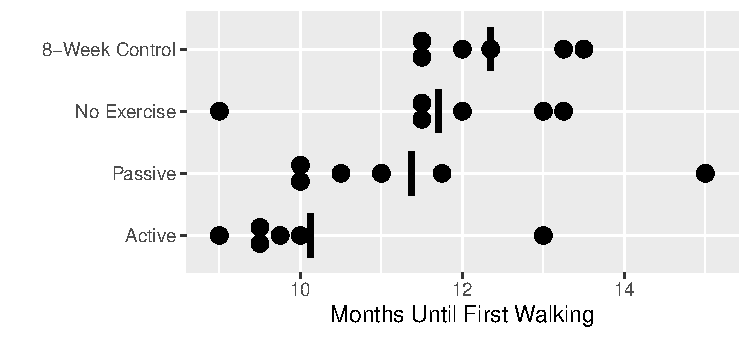
\includegraphics[width=\maxwidth]{multgroup-walking-1} }

\caption[Age of first walking]{Age in months when infants first began walking by treatment group with mean lines}\label{fig:multgroup-walking}
\end{figure}
\end{Schunk}
  \item Note that there are equal samples size in each group ($n_i =
    6$ for each $i$) in the example.  In general, this is not
    necessary for ANOVA, but it simplifies the calculations. 
  \item Thought process for ANOVA
   \bi
     \item Assume that age at first walk is Normally distributed with
       some variance $\sigma^2$ 
     \item The variance, $\sigma^2$, is unknown.  There are two ways
       of estimating $\sigma^2$ 
     \item Let the means in the four groups be $\mu_1$, $\mu_2$,
       $\mu_3$, and $\mu_4$ 
     \item Method 1
	\bi 
	  \item Assuming the variance are equal, calculated a pooled (or
      average) estimate of the variance using the four groups 
 	  \item $s^2_p = \frac{1}{4}(2.0938 + 3.5938 + 2.3104 + 0.7400) =
      2.184$ 
	\ei
     \item Method 2
	\bi 
	  \item Assuming the four treatments do not differ ($H_0: \mu_1 =
      \mu_2 = \mu_3 = \mu_4 = \mu$), the sample means follow a Normal
      distribution with variance $\sigma^2/6$. 
          \item We can then estimated $\sigma^2/6$ by the variance of
            the sample means ($s^2_{\overline{y}}$) 
          \item $s^2_{\overline{y}} = \textrm{variance of } {10.125,
              11.375, 11.708, 12.350}$ 
          \item $s^2_{\overline{y}} = 0.87349$, so $6
            s^2_{\overline{y}} = 5.247$ is our second estimate of
            $\sigma^2$ 
        \ei 
     \item $s^2_p$ is an estimate of the \textit{within} group variability
     \item $s^2_{\overline{y}}$ is an estimate of the \textit{among}
       (or \textit{between}) group variability 
     \item If $H_0$ is not true, method 2 will \textit{overestimate}
       the variance 
     \item The hypothesis test is based on $F = 6 s^2_{\overline{y}} /
       s^2_p$ and rejects $H_0$ if $F$ is too large 
   \ei
  \item Degrees of Freedom
   \bi 
     \item The $F$ statistic has both a numerator and denominator degrees of freedom
     \item For the numerator, d.f. = $k - 1$
       \bi 
          \item There are $k$ parameters ($\alpha_1, \alpha_2, \ldots,
            \alpha_k)$ 
          \item And \textit{one} restriction ($\Sigma \alpha_k = 0$,
            or $\alpha_1 = 0$, or another) 
       \ei
     \item For the denominator, d.f. = $N - k$
       \bi 
          \item There are $N$ total observations
          \item And we estimate $k$ sample means
       \ei
     \item In the age at first walking example, there are $3$ (numerator) and $20$ (denominator) degrees of freedom
   \ei
\begin{Schunk}
\begin{Sinput}
require(rms)
\end{Sinput}
\begin{Sinput}
f <- ols(months ~ trt, data=w)
anova(f)
\end{Sinput}
\begin{Soutput}
                Analysis of Variance          Response: months 

 Factor     d.f. Partial SS MS       F   P     
 trt         3   15.74031   5.246771 2.4 0.0979
 REGRESSION  3   15.74031   5.246771 2.4 0.0979
 ERROR      20   43.68958   2.184479           
\end{Soutput}
\end{Schunk}
\ei


\subsection{Connection to Linear Regression}
\bi
\item Can do ANOVA using multiple regression, using an intercept and
  $k-1$ ``dummy'' variables indicating group membership, so memorizing
  formulas specific to ANOVA is not needed
\item Why is between group d.f.=$k-1$?
 \bi
 \item can pick any one group as reference group, e.g., group 1
 \item $H_0$ is identical to
   $H_{0}:\mu_{2}-\mu_{1}=\mu_{3}-\mu_{1}=\ldots=\mu_{k}-\mu_{1}=0$
 \item if $k-1$ differences in means are all zero, all means must be
   equal
 \item since any unique $k-1$ differences define our goal, there is $k-1$
   d.f.\ between groups for $H_0$
 \ei
\ei

\section{Why All These Distributions?}
\bi
\item Normal distribution is handy for approximating the distribution
  of $z$ ratios (mean minus hypothesized value / standard error of
  mean) when $n$ is large or $\sigma$ is known
\item If $z$ is normal, $z^2$ has a $\chi^{2}_{1}$ distribution
\item If add $k$ $z^{2}$ values the result has a $\chi^{2}_{k}$
  distribution; useful
 \bi
 \item in larger than $2\times 2$ contingency tables
 \item in testing goodness of fit of a histogram against a theoretical
   distribution
 \item when testing more than one regression coefficient in regression
   models not having a $\sigma$ to estimate
 \ei
\item $t$ distribution: when $\sigma$ is estimated from the data;
  exact $P$-values if data from normal population \\
  Distribution indexed by d.f.: $t_{df}$; useful for
 \bi
 \item testing one mean against a constant
 \item comparing 2 means
 \item testing one regression coefficient in multiple linear regression
 \ei
\item $t_{df}^{2}$ has an $F$ distribution
\item $F$ statistic can test
 \bi
 \item $>1$ regression coefficient
 \item $>2$ groups
 \item whether ratio of 2 variances=1.0 (this includes MSB/MSW)
 \ei
\item To do this $F$ needs two different d.f.
 \bi
 \item numerator d.f.: how many unique differences being tested (like
   $\chi^{2}_{k}$)
 \item denominator d.f.
  \bi
  \item total sample size minus the number of means
   or regression coefficients and intercepts estimated from the data
  \item is the denominator of the estimate of $\sigma^2$
  \item also called the error or residual d.f.
  \ei
 \ei
\item $t_{df}^{2} = F_{1,df}$
\item ANOVA results in $F_{k-1,df}$; d.f.=$N-k$ where $N=$ combined
  total sample size; cf.\ 2-sample $t$-test: d.f.=$n_{1}+n_{2}-2$
\item Example: \ros{Ex.\ 12.4}
\beq
F = MSB/MSW = 58 \sim F_{4,1044}
\eeq
The cumulative probability of getting an $F$ statistic $\leq 58$ with
the above d.f.\ is 1.0000.  We want Prob$(F\geq 58)$, so we get
$P=1-1=0$ to several digits of accuracy but report $P<0.0001$.
\ei
\begin{Schunk}
\begin{Sinput}
pf(58, 4, 1044)
\end{Sinput}
\begin{Soutput}
[1] 1
\end{Soutput}
\begin{Sinput}
1 - pf(58, 4, 1044)
\end{Sinput}
\begin{Soutput}
[1] 0
\end{Soutput}
\end{Schunk}

\section{Software and Data Layout}
\bi
\item Every general-purpose statistical package does ANOVA
\item Small datasets are often entered using Excel
\item Statistical packages expect a grouping variable, e.g., a column
  of treatment names or numbers; a column of response values for all
  treatments combines is also present
\item If you enter different groups' responses in different spreadsheets or
  different columns within a spreadsheet, it is harder to analyze the
  data with a stat package
\ei

\section{Comparing Specific Groups} \ems{12.4}
\bi
\item $F$ test is for finding any differences but it does not reveal
  which groups are different
\item Often it suffices to quote $F$ and $P$, then to provide sample
  means (and their confidence intervals)
\item Can obtain CLs for any specific difference using previously
  discussed 2-sample $t$-test, but this can result in inconsistent
  results due solely to sampling variability in estimating the
  standard error of the difference in means using only the two groups
  to estimate the common $\sigma$
\item If assume that there is a common $\sigma$, estimate it using all
  the data \ros{Eq.\ 12.11}
  \\ to get a pooled $s^2$
\item $1-\alpha$ CL for $\mu_{i}-\mu_{j}$ is then
\beq
\bar{y}_{i}-\bar{y}_{j} \pm t_{n-k,1-\alpha/2} \times s
\sqrt{\frac{1}{n_{i}}+\frac{1}{n_{j}}},
\eeq
where $n$ is the grand total sample size and there are respectively
$n_{i}$ and $n_{j}$ observations in samples $i$ and $j$
\item Can test a specific $H_{0}: \mu_{i}=\mu_{j}$ using similar
  calculations; Note that the d.f.\ for $t$ comes from the grand
  sample size $n$, which $\uparrow$ power and $\downarrow$ width of
  CLs slightly
\item Many people use more stringent $\alpha$ for individual tests
  when testing more than one of them (Section \ref{multcomp})
 \bi
 \item This is not as necessary when the overall $F$-test is
   significant
 \ei
\ei

\section{Non-Parametric ANOVA: Kruskal-Wallis Test}
\bi
\item $k$-sample extension to the 2-sample Wilcoxon--Mann--Whitney
  rank-sum test
\item Is very efficient when compared to parametric ANOVA even if data
  are from normal distributions
\item Has same benefits as Wilcoxon (not harmed by outliers, etc.)
\item Almost testing for equality of population medians
\item In general, tests whether observations in one group tend to be
  larger than observations in another group (when consider randomly
  chosen pairs of subjects)
\item Test statistic obtained by replacing all responses by their
  ranks across all subjects (ignoring group) and then doing an ANOVA
  on the ranks
\item Compute $F$ (many authors use a $\chi^2$ approximation but $F$
  gives more accurate $P$-values)
\item Look up against the $F$ distribution with $k-1$ and $n-k$ d.f.
\item Very accurate $P$-values except with very small samples
\item Example: \ros{Ex.\ 12.21}
 \\ $F$ statistic from ranks in Table 12.16: $F_{3,20}=7.0289$
\item Using the cumulative distribution calculator from the web page,
  the prob.\ of getting an $F$ less impressive than this under $H_0$
  is 0.9979 \\
  $P$ is $1-0.9979=0.0021$
\item Compare with Rosner's $\chi^{2}_{3}=11.804$ from which $P=0.008$
  by \texttt{survstat} or one minus the CDF
\item Evidence that not all of the 4 samples are from the same
  distribution
 \bi
 \item loosely speaking, evidence for differences in medians
 \item better: some rabbits have larger anti-inflammatory effects
  when placed on different treatments in general
 \ei

\item Comparison of Kruskal-Wallis and Parametric ANOVA for age at
  first walk example 
 \bi
 \item A few extreme values in age a first walk may violate parametric
   $F$-test assumptions
 \item Run rank ANOVA: Kruskal-Wallis test three different ways:
   \bi
   \item Parametric ANOVA on the ranks of $y$
   \item Spearman's $\rho^2$ generalized to multiple columns of $x$
   \item An \R\ function dedicated to Kruskal-Wallis
   \ei
 \ei
\ei
\begin{Schunk}
\begin{Sinput}
anova(ols(rank(months) ~ trt, data=w))
\end{Sinput}
\begin{Soutput}
                Analysis of Variance          Response: rank(months) 

 Factor     d.f. Partial SS MS        F    P     
 trt         3   359.3333   119.77778 3.07 0.0515
 REGRESSION  3   359.3333   119.77778 3.07 0.0515
 ERROR      20   781.1667    39.05833            
\end{Soutput}
\begin{Sinput}
spearman2(months ~ trt, data=w)
\end{Sinput}
\begin{Soutput}

Spearman rho^2    Response variable:months

     rho2    F df1 df2      P Adjusted rho2  n
trt 0.315 3.07   3  20 0.0515         0.212 24
\end{Soutput}
\begin{Sinput}
kruskal.test(months ~ trt, data=w)
\end{Sinput}
\begin{Soutput}

	Kruskal-Wallis rank sum test

data:  months by trt
Kruskal-Wallis chi-squared = 7.2465, df = 3, p-value = 0.06444
\end{Soutput}
\end{Schunk}
Note that the classical Kruskal-Wallis test uses the $\chi^{2}$
approximation while the other two used an $F$ distribution, which is
as or more accurate than using $\chi^{2}$.

\section{Two-Way ANOVA} \ems{9.3}
\bi
\item Ideal for a factorial design or observational study with 2
  categorical grouping variables
\item Example: 3 treatments are given to subjects and the researcher
  thinks that females and males will have different responses in
  general \\
  Six means: $\bar{Y}_{i,j}, i=$ treatment, $j=$ sex group
\item Can test
 \bi
 \item whether there are treatment differences after
   accounting for sex effects
 \item whether there are sex differences after accounting for
   treatment effects
 \item whether the treatment effect is difference for females and
   males, if allow treatment $\times$ sex interaction to be in the
   model
 \ei
 \item Suppose there are 2 treatments ($A,B$) and the 4 means are
   $\bar{Y}_{Af}, \bar{Y}_{Bf}, \bar{Y}_{Am}, \bar{Y}_{Bm}$, where $f,
   m$ index the sex groups
 \item The various effects are estimated by
 \bi
 \item treatment effect: $\frac{(\bar{Y}_{Af}-\bar{Y}_{Bf})+(\bar{Y}_{Am}-\bar{Y}_{Bm})}{2}$
 \item sex effect: $\frac{(\bar{Y}_{Af}-\bar{Y}_{Am})+(\bar{Y}_{Bf}-\bar{Y}_{Bm})}{2}$
 \item treatment $\times$ sex interaction:
   $(\bar{Y}_{Af}-\bar{Y}_{Bf})-(\bar{Y}_{Am}-\bar{Y}_{Bm}) =
   (\bar{Y}_{Af}-\bar{Y}_{Am})-(\bar{Y}_{Bf}-\bar{Y}_{Bm})$
 \ei
\item Interactions are ``double differences''
\item Assessing whether treatment effect is same for $m$ vs.\ $f$ is
  the same as assessing whether the sex effect is the same for $A$
  vs.\ $B$
\item \textbf{Note}: 2-way ANOVA is \textbf{not} appropriate when one
  of the categorical variables represents conditions applied to the
  same subjects, e.g. serially collected data within patient with time
  being one of the variables; \\
  2-way ANOVA assumes that all observations come from different
  subjects
\ei

\section{Analysis of Covariance} \ems{12.5.3}
\bi
\item Generalizes two-way ANOVA
\item Allows adjustment for continuous variables when comparing groups
\item Can $\uparrow$ power and precision by reducing unexplained
  patient to patient variability ($\sigma^2$
\item When $Y$ is also measured at baseline, adjusting for the
  baseline version of $Y$ can result in a major reduction in variance
\item Fewer assumptions if adjust for baseline version of $Y$ using
  ANCOVA instead of analyzing ($Y -$ baseline $Y$)
\item Two-way ANOVA is a special case of ANCOVA where a categorical
  variable is the only adjustment variable (it is represented in the
  model by dummy variables)
\ei
See Chapter~\ref{chap:ancova} for much more information about ANCOVA
in RCTs.   % ???? TODO


\section{Multiple Comparisons}\alabel{multcomp} \ems{12.4.3}
\bi
\item When hypotheses are prespecified and are few in number, don't
  need to correct $P$-values or $\alpha$ level in CLs for multiple
  comparisons
\item Multiple comparison adjustments are needed with $H_{0}$ is
  effectively in the form 
 \bi 
 \item Is one of the 5 treatments effective when compared against
   control?
 \item Of the 4 etiologies of disease in our patients, is the
   treatment effective in at least one of them?
 \item Is the treatment effective in either diabetics, older patients,
   males, \ldots, etc.?
 \item Diabetics had the greatest treatment effect empirically; the
   usual $P$-value for testing for treatment differences in diabetics
   was 0.03 
 \ei
\item Recall that the probability that at least one event out of
  events $E_{1}, E_{2}, \ldots, E_{m}$ occurs is the sum of the
  probabilities if the events are mutually exclusive
\item In general, the probability of at least one event is $\leq$ the
  sum of the probabilities of the individual events occurring
\item Let the event be ``reject $H_0$ when it is true'', i.e., making
  a type I error or false positive conclusion
\item If test 5 hypotheses (e.g., 5 subgroup treatment effects) at the
  0.05 level, the upper limit on the chance of finding one significant
  difference if there are no differences at all is $5 \times 0.05 =
  0.25$
\item This is called the \emph{Bonferroni inequality}
\item If we test each $H_0$ at the $\frac{\alpha}{5}$ level the chance
  of at least one false positive is no greater than $\alpha$
\item The chance of at least one false positive is the
  \emph{experimentwise error probability} whereas the chance that a
  specific test is positive by chance alone is the
  \emph{comparisonwise error probability}
\item Instead of doing each test at the $\frac{\alpha}{m}$ level we can
  get a conservative adjusted $P$-value by multiplying an individual
  $P$-value by $m$\footnote{Make sure that $m$ is the total number of
    hypotheses tested with the data, whether formally or informally.}
\item Whenever $m \times P > 1.0$ report $P=1.0$
\item There are many specialized and slightly less conservative
  multiple comparison adjustment procedures.  Some more complex
  procedures are actually more conservative than Bonferroni.
\item Statisticians generally have a poor understanding about the need
  to not only adjust $P$-values but to adjust point estimates also,
  when many estimates are made and only the impressive ones (by $P$)
  are discussed.  In that case point estimates are badly biased away
  from the null value.  For example, the BARI study analyzed around 20
  subgroups and only found a difference in survival between PTCA and
  CABG in diabetics.  The hazard ratio for CABG:PTCA estimated from
  this group is far too extreme.
\ei
